\pdfminorversion=4
\documentclass[aspectratio=169]{beamer}

\mode<presentation>
{
  \usetheme{default}
  \usecolortheme{default}
  \usefonttheme{default}
  \setbeamertemplate{navigation symbols}{}
  \setbeamertemplate{caption}[numbered]
  \setbeamertemplate{footline}[frame number]  % or "page number"
  \setbeamercolor{frametitle}{fg=white}
  \setbeamercolor{footline}{fg=black}
} 

\usepackage[english]{babel}
\usepackage[utf8x]{inputenc}
\usepackage{tikz}
\usepackage{courier}
\usepackage{array}
\usepackage{bold-extra}
\usepackage{minted}
\usepackage[thicklines]{cancel}
\usepackage{fancyvrb}

\xdefinecolor{dianablue}{rgb}{0.18,0.24,0.31}
\xdefinecolor{darkblue}{rgb}{0.1,0.1,0.7}
\xdefinecolor{darkgreen}{rgb}{0,0.5,0}
\xdefinecolor{darkgrey}{rgb}{0.35,0.35,0.35}
\xdefinecolor{darkorange}{rgb}{0.8,0.5,0}
\xdefinecolor{darkred}{rgb}{0.7,0,0}
\definecolor{darkgreen}{rgb}{0,0.6,0}
\definecolor{mauve}{rgb}{0.58,0,0.82}

\title[2019-04-24-irishep-skyhook]{Skyhook for query systems}
\author{Jim Pivarski}
\institute{Princeton University -- IRIS-HEP}
\date{April 24, 2019}

\usetikzlibrary{shapes.callouts}

\begin{document}

\logo{\pgfputat{\pgfxy(0.11, 7.4)}{\pgfbox[right,base]{\tikz{\filldraw[fill=dianablue, draw=none] (0 cm, 0 cm) rectangle (50 cm, 1 cm);}\mbox{\hspace{-8 cm}
\includegraphics[height=1 cm]{princeton-logo-long.png}\hspace{0.1 cm}\raisebox{0.1 cm}{
\includegraphics[height=0.8 cm]{iris-hep-logo-long.png}}\hspace{0.1 cm}}}}}

\begin{frame}
  \titlepage
\end{frame}

\logo{\pgfputat{\pgfxy(0.11, 7.4)}{\pgfbox[right,base]{\tikz{\filldraw[fill=dianablue, draw=none] (0 cm, 0 cm) rectangle (50 cm, 1 cm);}\mbox{\hspace{-8 cm}
\includegraphics[height=1 cm]{princeton-logo.png}\hspace{0.1 cm}\raisebox{0.1 cm}{
\includegraphics[height=0.8 cm]{iris-hep-logo.png}}\hspace{0.1 cm}}}}}

% Uncomment these lines for an automatically generated outline.
%\begin{frame}{Outline}
%  \tableofcontents
%\end{frame}

% START START START START START START START START START START START START START

\begin{frame}{My view of the world}
\vspace{0.25 cm}
\begin{center}
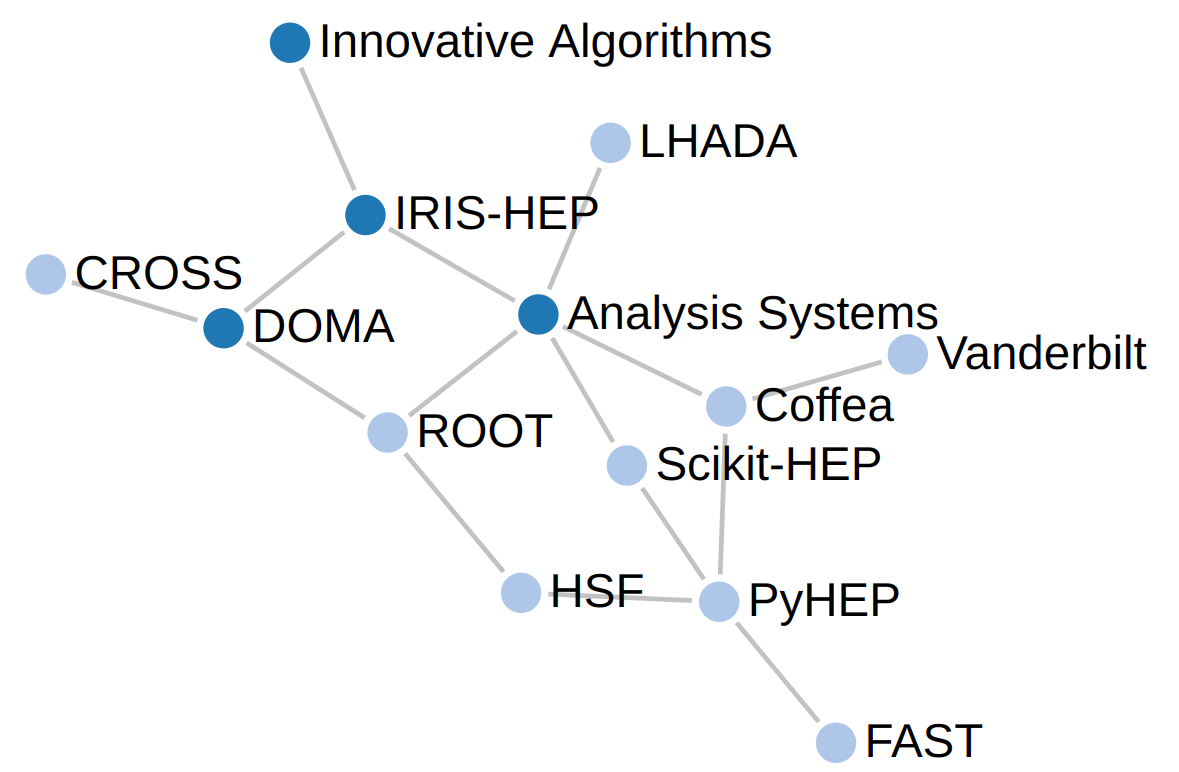
\includegraphics[width=0.8\linewidth]{analysis-connections-cross.png}
\end{center}

\scriptsize
\vspace{-2.5\baselineskip}
Biased? Incomplete? Help me fix it.

\textcolor{blue}{\url{https://github.com/iris-hep/analysis-connections}}
\end{frame}

\begin{frame}{Activities in Analysis Systems building toward an ntupleless future}
\vspace{0.5 cm}
\Large {\bf Query System:} big data on server, users request reduced output
\begin{center}
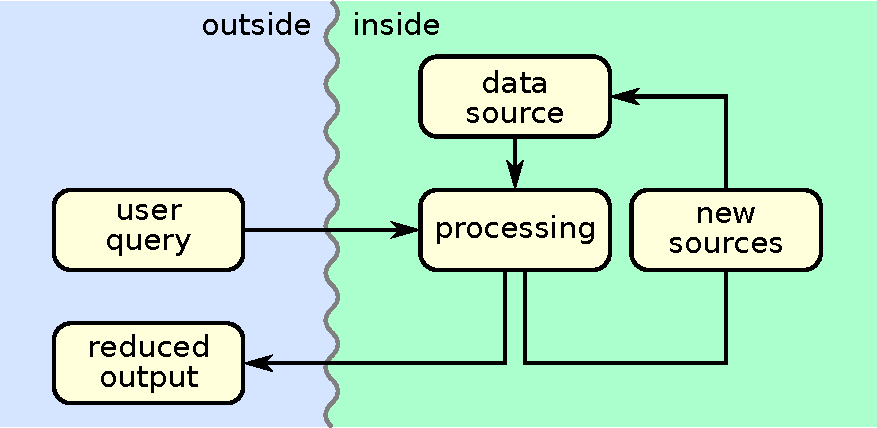
\includegraphics[width=0.6\linewidth]{basic-block-diagram.pdf}
\end{center}

\normalsize
\begin{itemize}
\item \textcolor{darkblue}{Mark Neubauer, Ben Galewsky:} query scheduling, data delivery, iDDS
\item \textcolor{darkblue}{Gordon Watts, Emma Torro, Mason Proffitt:} query expression language
\item \textcolor{darkblue}{Jim Pivarski, Henry Schreiner:} event data processing, histogram aggregation
\end{itemize}
\end{frame}

\begin{frame}{Feedback from analysis development}
\vspace{0.5 cm}
\begin{columns}
\column{0.2\linewidth}

\includegraphics[width=\linewidth]{coffea-logo.png}

\column{0.8\linewidth}
\hspace{-0.2 cm}\Huge Coffea

\vspace{0.25 cm}
\large {\bf C}olumnar {\bf O}bject {\bf F}ramework {\bf F}or {\bf E}fficient {\bf A}nalysis

\vspace{0.25 cm}
\normalsize Matteo~Cremonesi, Lindsey~Gray, Oliver~Gutsche, Allison~Hall, Bo~Jayatilaka, Igor~Mandrichenko, Kevin~Pedro, Nick~Smith~[FNAL]
\end{columns}

\begin{center}
\begin{minipage}{0.8\linewidth}
\large Performing two complete CMS analyses
\begin{itemize}
\item Dark Higgs search
\item Boosted SM $H \to b\bar{b}$
\end{itemize}
using my \textcolor{darkblue}{awkward-array}, Ben's \textcolor{darkblue}{distributed processing with Spark}, and Andrew Melo's \textcolor{darkblue}{Spark cluster at Vanderbilt}.
\end{minipage}
\end{center}
\end{frame}

\end{document}
